\documentclass[11pt]{article}
\usepackage[T1,T2A]{fontenc}
\usepackage[utf8]{inputenc}
\usepackage[english,russian]{babel}
\usepackage{graphicx}
\usepackage{amsmath}
\graphicspath {{img/}}
\title{\textbf{Лабораторная работа №7\\
<<Помехоустойчивое кодирование. Мажоритарное декодирование>>}}
\author{Матяш А.А., ККСО-01-19}
\date{}
\addtolength{\topmargin}{-3cm}
\addtolength{\textheight}{3cm}
\begin{document}
\maketitle
\thispagestyle{empty}
\textbf{Цель работы:} ознакомление с принципами построения систем передачи с мажоритарным декодированием и приобретение практических навыков постановки и проведения исследований.\\
Для линейных кодов, рассчитанных на исправление многократных ошибок, часто более простыми оказываются декодирующие устройства, построенные по мажоритарному принципу.\\ 
\indentИдея мажоритарного декодирования линейного кода базируется на системе проверочных равенств, а именно, в кодах с мажоритарным декодированием, каждый символ может быть выражен через другие символы несколькими способами. Это позволяет для определения истинного значения символа воспользоваться принципом большинства (мажоритарным принципом).\\
\indentЛюбой символ $a_{i}$, выражается $d$ (минимальное кодовое расстояние) различными независимыми способами в виде линейных комбинаций других символов. Результаты вычислений подаются на соответствующий этому символу мажоритарный элемент. Последний представляет собой схему, имеющую d входов и один выход, на котором появляется единица, когда возбуждается больше половины его входов, и нуль, когда возбуждается число таких входов меньше половины. Если ошибки отсутствуют, то проверочные равенства не нарушаются, и на выходе мажоритарного элемента получаем истинное значение символа. Рассмотрим процесс мажоритарного декодирования на примере. Пусть передано кодовое слово $(8,2)$ линейного кода:\\
\begin{center}
    $U = (u_{8}, u_{7}, u_{6}, u_{5}, u_{4}, u_{3}, u_{2}, u_{1})$
\end{center}
символы которого сформированы в соответствии с системой проверочных уравнений (правилом кодирования) на основе информационных бит $(a_{2},a_{1})$ вида:
\begin{center}
    $u_{8} = a_{2}, u_{7} = a_{2}, u_{6} = a_{2}, u_{5} = a_{1}, u_{4} = a_{1}, u_{3} = a_{1}, u_{2} = a_{1} \oplus a_{2}, u_{8} = a_{1} \oplus a_{2}$
\end{center}
На входе декодера наблюдается принятая последовательность:
\begin{center}
    $R = (r_{8}, r_{7}, r_{6}, r_{5}, r_{4}, r_{3}, r_{2}, r_{1})$
\end{center}
и необходимо ее декодировать, то есть определить оценки передаваемой информационной последовательности $(a_{2}^{*},a_{1}^{*})$.\\
\indentДля начала предположим, что ошибок в принятой последовательности R нет, тогда по принятой последовательности R можно легко найти оценку переданной информационной последовательности $(a_{2}^{*},a_{1}^{*})$, причем не единственным способом:
\begin{center}
    $a_{1}^{*}=r_{1}\oplus r_{6},a_{1}^{*}=r_{2}\oplus r_{7}, a_{1}^{*}=r_{3}, a_{1}^{*}=r_{4}, a_{1}^{*}=r_{5}$\\
    $a_{2}^{*}=r_{1}\oplus r_{3}, a_{2}^{*}=r_{2}\oplus r_{4}, a_{2}^{*}=r_{6}, a_{2}^{*}=r_{7}, a_{2}^{*}=r_{8}.$
\end{center}
\indentТаким образом, получилось пять независимых систем уравнений для определения одних и тех же компонент $(a_{2}^{*}, a_{1}^{*})$, причем, они будут иметь одинаковые решения только при отсутствии ошибок в принятой последовательности r. 
\indentВ противном случае решения для $(a_{2}^{*},a_{1}^{*})$, даваемые различными системами, будут разными. \\
\indentЕсли считать, что в принятой последовательности возможна только одиночная ошибка, то ошибочным будет решение одного уравнения из пяти для каждого из элементов $(a_{2}^{*},a_{1}^{*})$, остальные четыре уравнения дадут правильное решение. Тогда правильный ответ может быть получен по «большинству голосов».\\
\indentВ ходе лабораторной работы рассмотрена 1 задача:\\
\indentИсследование системы передачи c мажоритарным декодированием группового (8,2)-кода.\\
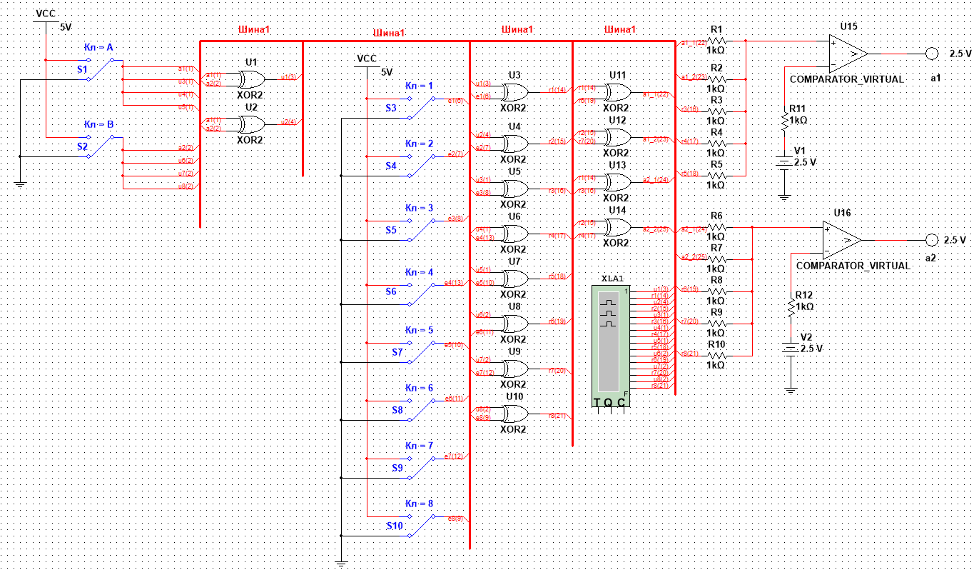
\includegraphics[width=1\linewidth]{scheme.png}
\newpage
\indentДаны информационные биты $a_{2} a_{1}=01$. Они преобразуются в кодовое слово $U=(u_{8},u_{7},u_{6},u_{5},u_{4},u_{3},u_{2},u_{1} )=(a_{2},a_{2},a_{2},a_{1},a_{1},a_{1},a_{1}\oplus\\ \oplus a_{2},a_{1}\oplus a_{2})=00011111$. Выполним моделирование при отсутствии и наличии ошибок, результаты зафиксируем в таблице:\\
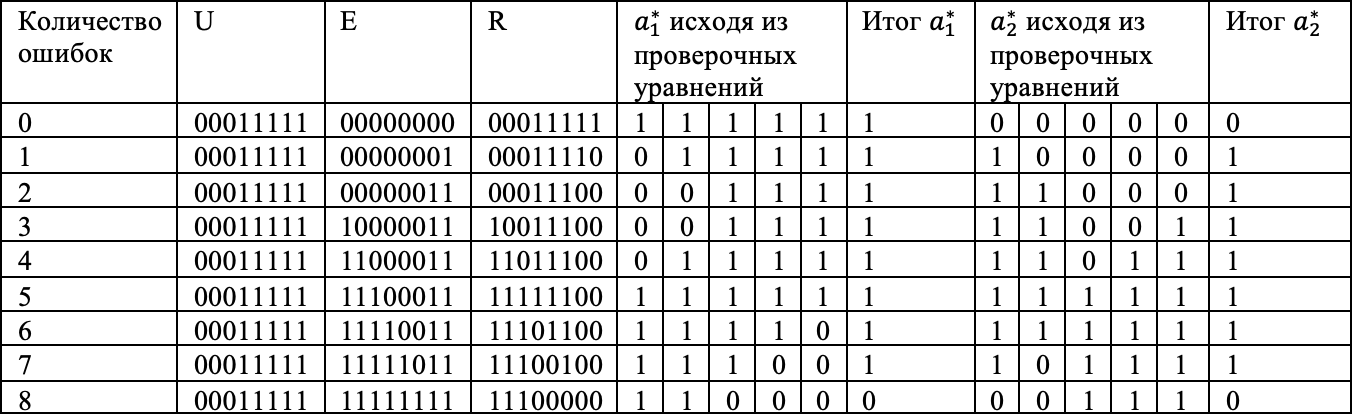
\includegraphics[width=1\linewidth]{table.png}
\indentИсходя из таблицы делаем вывод, что мажоритарное декодирование эффективно справляется с ошибками, если их количество менее трёх. В противном случае происходит искажение переданной информации.\\
\textbf{Вывод:} в ходе работы я ознакомился с принципами построения систем передачи с мажоритарным декодированием, а также приобрёл практические навыки постановки и проведения исследований.
\end{document}

